% Cap�tulo 5
\chapter{Experimentos}


Após realizar as implementações dos métodos, esse capítulo busca comparar as duas soluções através da realização de testes com o objetivo de saber qual delas é a mais oritimizada. Para tanto, a máquina utilizada no experimento apresenta as seguintes configurações: 


\begin{itemize}
    \item Sistema operacional: Windows 10 (64 bits);
    \item Processador: Intel Core i7-7500U com 3.5 GHz;
    \item Memória RAM: 8 Gigabytes;
\end{itemize}

Para auxiliar no desenvolvimento e execução, foi utilizado o ambiente de desenvolvimento integrado NetBeans na versão 8.2.

\section{Testes}

A execução dos testes levou em consideração de 1 a 100.000 embaralhamentos distintos. Cada um deles foram gerados de maneira aleatória, realizando um total de 40 giros. Tanto no método em camadas quanto no Fridrich foram avaliadas as seguintes quantidades de configurações: 

\begin{itemize}
    \item 1º teste: 1 configuração;
    \item 2º teste: 10 configurações;
    \item 3º teste: 100 configurações;
    \item 4º teste: 1.000 configurações;
    \item 5º teste: 5.000 configurações;
    \item 6º teste: 10.000 configurações;
    \item 7º teste: 50.000 configurações;
    \item 8º teste: 100.000 configurações.
    
\end{itemize}


\subsection{Análise do tempo de execução}
A análise do tempo é medida em segundos, considerando quatro casas decimais. Para cada teste os algoritmos foram executados duas vezes e a partir dos tempos colhidos foram efetuadas as médias. A seguir é mostrada a tabela com os tempos obtidos:

\begin{table}[!htb]   
    \textsf{\caption{Análise do tempo}}
    \centering
    \medskip
   
    \begin{tabular}{c|c|c}  
        \hline
        \textbf{Embaralhamentos} & 
        \textbf{Método em Camadas} &
        \textbf{Método de Fridrich} \\
        \hline
        1 & 0,0160 & 0,0160   \\
        \hline
        10 & 0,0780 & 0,1080   \\
        \hline
        100 & 0,7110 & 0,6700   \\
        \hline
        1.000 & 5,1090 & 5,6840 \\
        \hline
        5.000 & 27,8940 & 25,4500 \\
        \hline
        10.000 & 51,4280 & 47,4030 \\
        \hline
        50.000 & 224,3380 & 211,8780 \\
        \hline
        100.000 & 463,0010 & 448,8560 \\
        \hline
        
    \end{tabular}
    \label{table:tab1}
\end{table}


\begin{figure}[!htb]
    \centering
    {
        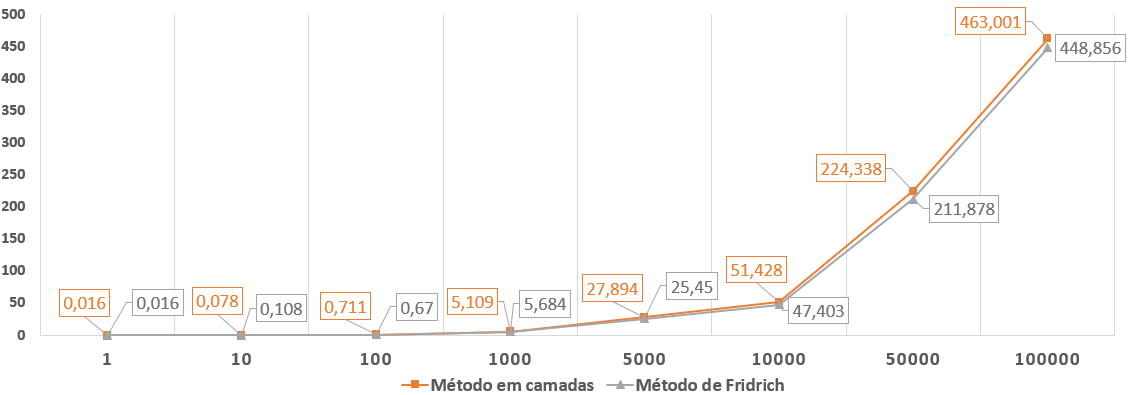
\includegraphics[height=5.2cm]{imagens/graficoFinal3.png}
        \label{figFront}
    }
    
\caption{Tempos de execução}
\label{fig:figconceiBlo}
\legend{Fonte: Elaborado pelo autor (2017)}
\end{figure}


Na primeira linha da Tabela 5 estão os tempos obtidos na execução das duas soluções para apenas uma configuração do cubo de Rubik, que, nesse caso, são idênticos. A partir de 10 embaralhamentos, já é possível ver a diferença nos tempos, com o Fridrich obtendo um tempo de 0,03 segundo a mais que o método em camadas, conforme é mostrado na segunda linha. 

O tempo do Fridrich mostra-se mais eficiente quando o algoritmo é executado 100 vezes, no entanto, quando essa quantidade aumenta para 1.000, o tempo do método em camadas passa a ser menor, com uma diferença de 0,575 segundo.


A partir de 5.000 embaralhamentos, o Fridrich claramente apresenta um desempenho melhor, executando com uma diferença de 2,444 segundos (10\% mais rápido). Esse comportamento é mantido quando ampliamos para 10.000, 50.000 e 100.000 embaralhamentos, com uma diferença no tempo de 4,025 (8\%), 12,46 (6\%) e 14,145 (3\%) segundos, respectivamente.

No geral, o método de Fridrich tende a ser mais performático no seu tempo de execução a medida que o número de embaralhamentos aumenta. Como dito acima, essa diferença torna-se mais evidente quando os algoritmos são executados a partir de 5.000 configurações distintas. O gráfico da Figura \ref{fig:figconceiBlo} ilustra a evolução dos tempos nos dois algoritmos.




\subsection{Análise do número de movimentos}

Outro parâmetro analisado é a quantidade média de movimentos gerada por cada solução. Na avaliação realizada no capítulo 2, ficou claro que o método de Fridrich é mais avançado que outras técnicas porque possui mais algoritmos que objetivam montar mais de uma camada simultaneamente, gerando, assim, menos movimentos quando comparado com outras soluções. Esse fato foi provado nesta análise, como mostra a tabela abaixo.


\begin{table}[!htb]   
    \textsf{\caption{Análise de tempo}}
    \centering
    \medskip
   
    \begin{tabular}{c|c|c}  
        \hline
        \textbf{Embaralhamentos} & 
        \textbf{Método em Camadas} &
        \textbf{Método de Fridrich} \\
        \hline
        1 & 124 & 103   \\
        \hline
        10 & 104 & 72   \\
        \hline
        100 & 101 & 71   \\
        \hline
        1.000 & 100 & 73 \\
        \hline
        5.000 & 100 & 72 \\
        \hline
        10.000 & 100 & 72 \\
        \hline
        50.000 & 100 & 72 \\
        \hline
        100.000 & 100 & 72 \\
        \hline
        
    \end{tabular}
    \label{table:tab1}
\end{table}

Ao analisar a Tabela 6, a primeira linha mostra a quantidade média de movimentos que soluciona apenas uma configuração do cubo de Rubik, com uma diferença de 21 movimentos a menos quando executada pelo método de Fridrich. Com 10 embaralhamentos, essa diferença aumenta para 32.

Executando cada algoritmo 100 vezes, o Fridrich continua performático, realizando 30 movimentos a menos. Quando chegamos em 1.000 embaralhamentos, o método em camadas gera uma média de 100 movimentos, que se mantém constante para 5.000, 10.000, 50.000 e 100.000. A partir de 5.000 execuções, a diferença de movimentos passa a ser 28.   

Em suma, o Fridrich realiza, em média, quase 30 movimentos a menos do que o método em camadas. Em alguns casos pode executar ainda menos movimentos utilizando giros considerados avançados, como, por exemplo, mover duas faces ao mesmo tempo.

Diante dos resultados obtidos pelos testes, é evidente que o método de Fridrich, tanto na análise do seu tempo de execução quanto na quantidade de movimentos, é, de fato, uma técnica otimizada para solucionar o cubo de Rubik.


\section{Estudo de caso}


A fim de melhor entender a diferença entre as duas soluções, é essencial realizar uma análise específica para demonstrar as diferenças de cada algoritmo. Em vista disso, uma configuração foi selecionada (Figura \ref{fig:emba}) com o intuito de apresentar a saída esperada no método em camadas e no Fridrich.


\begin{figure}[!htb]
    \centering
    {
        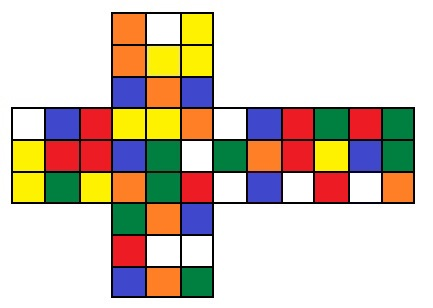
\includegraphics[height=5cm]{imagens/emba2.jpg}
        \label{figFront}
    }
    
\caption{Embaralhamento}
\label{fig:emba}
\legend{Fonte: Elaborado pelo autor (2017)}
\end{figure}


Na solução da configuração ilustrada na figura \ref{fig:emba}, o método em camadas realiza, no primeiro passo, 12 movimentos. Nesse ponto inicial, os dois algoritmos apresentam o mesmo desempenho, uma vez que a primeira etapa do método de Fridrich é exatamente a mesma do método de camadas. Os giros realizados são: R’, D’, U’, L2, B, U, R, B2, R2, B, U e R2.


Para fazer o posicionamento das quatro peças de quina da primeira camada são realizados 19 movimentos utilizando o método em camadas: R, U’, R’, U, R, U’, R’, L’, U, L, U’, L’, U, L, B, U, B2, U2 e B. Já no passo seguinte, orientação das peças de meio da segunda camada, são efetuados 41 giros: U’, F’, U, F, U, R, U’, R’, B’, U’, B, U, F, U’, F’, U’, L’, U, L, B’, U, B, L, U, L’, U2, L, U2, L’, U, B’, U’, B, U, B, U’, B’, U’, R’, U e R.

É importante notar que, através do método em camadas, os dois passos anteriores contabilizam um total de 60 giros. Utilizando o método de Fridrich essa quantidade apresenta uma redução significativa, totalizando 35 giros: U’, B, U’, B’, U, B, U, B’, U2, F, U, F’, U2, L’, U, L, U, L, U’, L’, U2, L, U’, L’, R, U’, R’, U’, R, U, R’, U2, R, U’ e R’.

O método em camadas realiza 11 movimentos para fazer a cruz na face do topo e 7 para orientar as peças de quina, totalizando 18 movimentos: F, R’, F’, R, U2, F, R’, F’, R2, U2, R’, R, U2, R’, U’, R, U’ e R’. Para efetuar esses mesmos passos, que chamamos de OLL, o Fridrich realiza apenas 8 giros: L, F, R’, F’, L’, F, R e F’.

Os dois últimos passos, permutação das peças de quina e de meio da face U, resultam em 26 movimentos: U2, R’, F, R’, B2, R, F’, R’, B2, R2, U’, R’, U’, R’, F, R, F’, U, R, F’, U’, L’, U, L, F e U. No Fridrich, por sua vez, essas duas etapas são realizadas pelos algoritmos do F2L, gerando apenas 10 giros: R’, F, R’, B2, R, F’, R’, B2, R2 e U.

Como podemos constatar, há uma considerável redução no número de movimentos quando solucionamos o cubo de Rubik através do método de Fridrich. Contabilizando todos os giros efetuados para solucionar o cubo, o método em camadas gerou um total de 116 giros, enquanto que utilizando o método de Fridrich há redução de 51 giros, contabilizando 65 movimentos para solucioná-lo por completo.

\section{Análise da complexidade}

A análise da complexidade de algoritmo reflete diretamente no esforço computacional requerido para executá-lo. Esse esforço computacional mede a quantidade de trabalho, em termos de tempo de execução ou da quantidade de memória requerida \cite{toscale}.

Uma maneira interessante de aferir o esforço computacional é utilizando a análise matemática. Essa análise não depende da implementação do algoritmo e pode ser aferida na fase de projeto de algoritmo \cite{toscale}.

A notação Big-O descreve o comportamento geral do algoritmo em termos do crescimento do número de operações conforme cresce o número de elementos processados. Com base na notação Big-O tanto o método em camadas quanto o método de Fridrich apresentam complexidade O(n), onde n é o número de peças que estão incorretamente posicionadas, podendo ser peça de quina ou de meio. O valor de n varia de acordo com a quantidade de peças que não estão posicionadas corretamente.
